\documentclass{article}
\usepackage{geometry}
\usepackage{graphicx}

\geometry{
a4paper,
right=10mm,
left=10mm,
top=10mm,
bottom=10mm,	
}

\begin{document}

\pagenumbering{gobble}

\begin{center}
\textbf{\Large Programming Assignment 4} \\
\textit{\large Jayant Agrawal}         14282 \\
\textit{\large Shubham Pandey}         14679
\end{center}

\section{Quick Sort versus Merge Sort}

No of iterations : 2000
\begin{center}
\begin{tabular}{||c|c|c|c|c|c||}
\hline
 		&  $n=10^2$ & $n=10^3$ &$n=10^4$  & $n=10^5$ &$n=10^6$   \\
\hline
Average running time of Quick Sort(s) &
0.000006&
0.000090&
0.001187&
0.014851&
0.178958\\
\hline
Average running time of Merge Sort(s) &
0.000007&
0.000102&
0.001330&
0.016136&
0.195267 \\
\hline
Average number of comparisons during Quick Sort & 
645.35&
10980.48&
155472.53&
2016323.09&
24766309.45 \\
\hline
The value of $1.39nlog_{2}n$ & 923 & 13852.44 &184699.20 &2308740.02 &27704880.31 \\ 
\hline
Average number of comparisons during Merge Sort&
541.97&
8707.60&
120454.70&
1536395.64&
18674389.63\\
\hline
The value of $nlog_{2}n$ & 664.38 &9965.78 &132877.12 &1660964.04 &19931568.57 \\
\hline
Number of times Merge Sort outperformed Quick Sort & 22 &35 &5 &3 & 2 \\
\hline
\end{tabular}
\end{center}

\subsection{Inference}
\begin{itemize}
\item Number of Comparisons in Quick Sort are more than Merge Sort, but still Quick Sort takes less time, for all n.
	\begin{itemize}
	\item Merge Sort takes time for copying data from the temporary array to the original array.
	\item For Quick sort almost half of the comparisons do not initiate any further operation (swapping, copying etc).
	\end{itemize}
\item Merge Sort may perform better when it is used on linked lists, where memory manipulations are easier and faster.
\item With increasing n, the probability of tha sample being close to the worst case sample for quick sort reduces, so does the probability of merge sort outperforming quick sort.
\end{itemize}


%Number of Comparisons in quick sort are more, but still it performs better because in merge sort data copying takes more time. Also, in quick sort in almost half of the comparisons,we don't have to swap. So, merge sort may perform better in linked lists. As n increases, the probability of getting the worst case sample for quick sort reduces, so does the probability of merge sort outperforming quick sort. 


\section{Distribution of the running time of Quick Sort}

No of iterations : 2000
\subsection{Table}

\begin{center}
\begin{tabular}{||c|c|c|c|c|c||}
\hline
 		&  $n=10^2$ & $n=10^3$ &$n=10^4$  & $n=10^5$ &$n=10^6$   \\
\hline
Average running time of Quick Sort(s)($\mu$) &
0.000006&
0.000090&
0.001187&
0.014851&
0.178958\\
\hline
$1.39nlog_{2}n$ & 923 & 13852.44 &184699.20 &2308740.02 &27704880.31 \\ 
\hline
Average number of comparisons during Quick Sort & 
645.35&
10980.48&
155472.53&
2016323.09&
24766309.45 \\
\hline
\# cases where run time exceeds average by 5\% & 638& 253&259 &198 &204 \\
\hline
\# cases where run time exceeds average by 10\% & 638&89 & 30& 8&26 \\
\hline
\# cases where run time exceeds average by 20\% & 101& 48& 5& 2& 0\\
\hline
\# cases where run time exceeds average by 30\% & 101&25 & 1&1 & 0\\
\hline
\# cases where run time exceeds average by 50\% & 48& 10& 0& 0& 0\\
\hline
\# cases where run time exceeds average by 100\% & 15& 0& 0& 0& 0\\
\hline
\end{tabular}
\end{center}

\subsubsection{Inference}
\begin{center}
\begin{tabular}{||c|c|c|c|c|c||}
\hline
        &  $n=10^2$ & $n=10^3$ &$n=10^4$  & $n=10^5$ &$n=10^6$   \\
	\hline	
Variance($\sigma^2$) &$2.7\times10^{-9}$ &$6.18\times10^{-8}$ & $1.98\times10^{-6}$&$2.05\times10^{-4}$ & 0.036\\
\hline
Coefficient of Restitution ($C_{X}$)($\sigma/\mu$) &8.66 & 2.76 & 1.16 & 0.96 &1.0  \\
\hline
\end{tabular}
\end{center}

\begin{itemize}
\item For a given 'n', no of cases decreases as we move away from average showing that the probability of the worst case is very low.
\item For increasing 'n', no of cases exceeding a given \% above $\mu$ decreases showing that the run time moves further closer to the average value.
\item As n increases, $C_{X}$ decreases, which further confirms the fact that for a large data size the distribution of the running time gets sharper with mode being closer to the average.
\end{itemize}
    
\subsection{Plots}
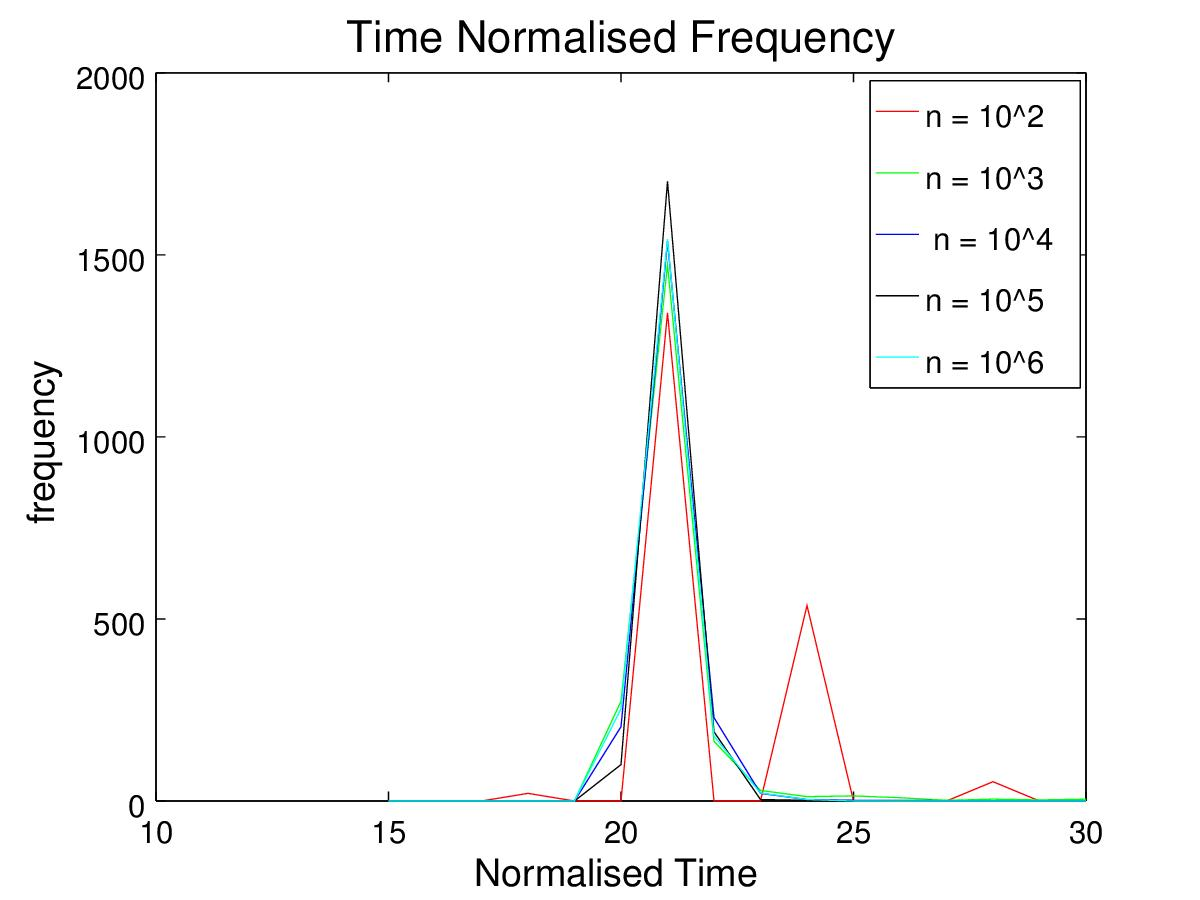
\includegraphics[width=1\columnwidth]{plot2.jpg}\\

\subsubsection{Plot Description}
For each 'n', taking 5\% of the average as the bin size for the histogram, frequency vector is calculated. Then, all such vectors are plotted on the graph.
The x-range is 10-30 for better pictorial representation.
\subsubsection{Inference}
\begin{itemize}
\item For smaller 'n' value, the plot shows relatively lesser sharpness, showing that for small n , the probability for the sample to be closer to the worst case is higher.(But, this does not matter, since for small 'n' run time is already very less).
\item As evident from the graph, that the peak of the plot is higher for greater 'n'. This implies that for increasing 'n', frequency near average increases.
\end{itemize}

\section{Further Observations}
\begin{enumerate}
\item Theoretically we have calculated the time complexity based on no of comparisons, but we have ignored the time taken in memory input/output.
In quick sort,we are comparing with the same pivot element, whereas in merge sort we are comparing different elements.
The cache is utilised well in the case of quick sort.
\item The worst case time for quick sort is $O(n^2)$. Some of the cases where this happens, can be improved with better selection of pivot(randomized or median).
Moreover, if the data can be randomized initially to avoid the worst case(sorted array) for quick sort.
\item For any 'n', the probability of the sample being sorted is $1/(n!)$. So, for larger 'n' , it is less likely to get the worst case for quick sort.
\end{enumerate}
\end{document}


